\documentclass{standalone}
\usepackage{tikz}
\usepackage{pgfplots}
\pgfplotsset{compat=1.18}
\usepgfplotslibrary{fillbetween}      % <-- needed for fill between
\usetikzlibrary{arrows.meta,decorations.pathreplacing,calligraphy}
\usepackage{amsmath}
\usepackage{sansmath}

\usepackage[T1]{fontenc}
\usepackage{newtxtext}
\usepackage{newtxmath}

\definecolor{mblue}  {RGB}{0,   114, 189}
\definecolor{morange}{RGB}{217,  83,  25}
\definecolor{mgreen} {RGB}{119, 172,  48}
\definecolor{mpurple}{RGB}{126,  47, 142}

%% ── Bézier expressions (reused in both passes via macros) ───────────────
\def\cubicX{ 0.15+ 7.989*(1-\t)^2*\t + 14.625*(1-\t)*\t^2 + 6.500*\t^3}
\def\cubicY{ -1.038*(1-\t)^2*\t + 13.260*(1-\t)*\t^2 + 4.767*\t^3}

\def\quinticX{ 0.15+
    17.040*(1-\t)^4*\t
  -  1.320*(1-\t)^3*\t^2
  + 28.150*(1-\t)^2*\t^3
  + 17.665*(1-\t)*\t^4
  +  5.950*\t^5}
\def\quinticY{
  -  1.900*(1-\t)^4*\t
  + 44.810*(1-\t)^3*\t^2
  +  5.300*(1-\t)^2*\t^3
  + 22.905*(1-\t)*\t^4
  +  5.500*\t^5}

%% ── Fill x-limits (edit only these two lines) ──────────────────────────
\def\xfillL{2.2}      % left  boundary (x-coordinate)
\def\xfillR{3.5}   % right boundary (x-coordinate) = x_T
%% ─────────────────────────────────────────────────────────────────────
\newcommand{\fsize}{\fontsize{8.7}{10.44}\selectfont}

\begin{document}
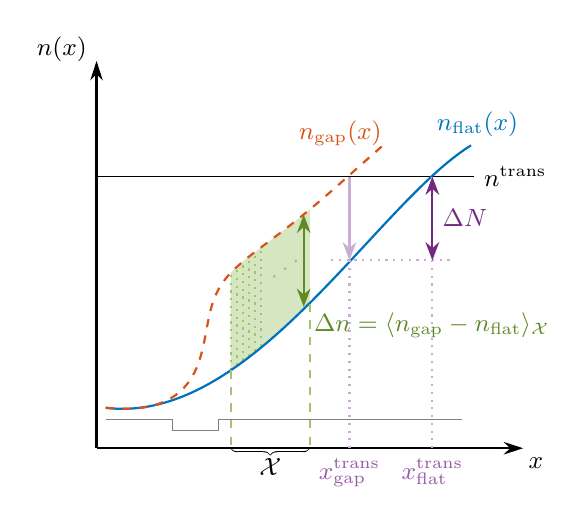
\begin{tikzpicture}
	\begin{axis}[
		width=7cm, height=6.5cm,
		xmin=0, xmax=7.0,
		ymin=-0.7, ymax=6.0,
		axis lines=left,
		xlabel={$x$},
		xlabel style={
				at={(axis description cs:1.03,0)},
				anchor=north},
		ylabel={$n(x)$},
		ylabel style={
				at={(axis description cs:0,1.03)},
				anchor=east, rotate=-90},
		xtick=\empty, ytick=\empty,
		axis line style={thick, -{Stealth[length=7pt,width=4.5pt]}},
		clip=false,
		font=\fsize,
		]

		%% ── A_T reference line ──────────────────────────────────────────────────
		\addplot[thin, black, no markers]
		coordinates {(0,4.0)(6.2,4.0)}
		node[pos=1, right] {$n^{\text{trans}}$};

		%% ── Pass 1 : invisible named paths (geometry only, used by fillbetween) ─
		\addplot[draw=none, name path=curveA,
			domain=0:0.90, samples=200, variable=\t]
		({\cubicX},   {\cubicY});

		\addplot[draw=none, name path=curveB,
			domain=0:0.88, samples=300, variable=\t]
		({\quinticX}, {\quinticY});

		%% ── Fill between the two curves, clipped to x ∈ [\xfillL, \xfillR] ────
		\addplot[mgreen, fill opacity=0.3, draw=none]
		fill between[
				of=curveA and curveB,
				soft clip={domain=\xfillL:\xfillR},
			];

		\def\mA{0.83}
		\def\mB{0.8}
		\draw[mgreen!70,thick, dotted](axis cs:\xfillL,0.65) -- (axis cs:\xfillL,2.35);
		\draw[mgreen!70,thick, dotted](axis cs:\xfillL+0.1,0.65+\mA*0.1) -- (axis cs:\xfillL+0.1,2.35+\mB*0.1);
		\draw[mgreen!70,thick, dotted](axis cs:\xfillL+0.2,0.65+\mA*0.2) -- (axis cs:\xfillL+0.2,2.35+\mB*0.2);
		\draw[mgreen!70,thick, dotted](axis cs:\xfillL+0.3,0.65+\mA*0.3) -- (axis cs:\xfillL+0.3,2.35+\mB*0.3);
		\draw[mgreen!70,thick, dotted](axis cs:\xfillL+0.4,0.65+\mA*0.4) -- (axis cs:\xfillL+0.4,2.35+\mB*0.4);
		\draw[mgreen!70,thick, dotted](axis cs:\xfillL+0.5,0.65+\mA*0.5) -- (axis cs:\xfillL+0.5,2.35+\mB*0.5);
		\draw[mgreen!70,thick, loosely dotted, yshift=-0.1cm](axis cs:2.9,2.4) -- (axis cs:3.3,2.7);

		\addplot[mblue, thick,
			domain=0:0.90, samples=200, variable=\t, smooth]
		({\cubicX}, {\cubicY});

		\addplot[morange, thick, dashed,
			domain=0:0.87, samples=300, variable=\t, smooth]
		({\quinticX}, {\quinticY});
		\draw[mpurple!40, thick, dotted]
		(axis cs:4.15,-0.7) -- (axis cs:4.15,4.0)
		node[mpurple!80,pos=0, below] {$x_\text{gap}^{\text{trans}}$};
		\draw[mpurple!40, thick, dotted]
		(axis cs:5.51,-0.7) -- (axis cs:5.51,4.0)
		node[mpurple!80,pos=0, below] {$x_\text{flat}^{\text{trans}}$};
		\draw[mpurple!40, thick, Stealth-]
		(axis cs:4.15,2.55) -- (axis cs:4.15,4.0);
		\draw[mpurple!40, thick, dotted]
		(axis cs:3.85,2.55) -- (axis cs:5.85,2.55);
		\draw[mpurple!90!black, thick, Stealth-Stealth]
		(axis cs:5.51,2.55) -- (axis cs:5.51,4.0)
		node[pos=0.5, right] {$\Delta N$};
		\begin{scope}[yshift=0cm]
			\draw[black, opacity=0.5, thin] (axis cs:0.15,-0.2) -- (axis cs:1.25,-0.2) -- (axis cs:1.25,-0.4) -- (axis cs:2,-0.4) -- (axis cs:2,-0.2) -- (axis cs:6,-0.2);
		\end{scope}

		\draw[mgreen!80!black,thick, Stealth-Stealth]	(axis cs:\xfillL+1.2,0.65+\mA*1.2+0.1) -- (axis cs:\xfillL+1.2,2.4+\mB*1.2-0.02)
		node[pos=0-0.2, right] {$\Delta n= \langle n_\text{gap}-n_\text{flat}\rangle_{\mathcal{X}}$};
		\draw[mgreen!70,dashed, thick] (axis cs:\xfillL,0.65) -- (axis cs:\xfillL,-0.7);
		\draw[mgreen!70,dashed, thick] (axis cs:\xfillR,1.8) -- (axis cs:\xfillR,-0.7);
		% \draw[mgreen!80!black,thick,{Bracket[sharp]-Bracket[sharp]}]	(axis cs:\xfillL,-0.7) -- (axis cs:\xfillR,-0.7)
		% 	node[pos=0.5, below] {$\mathcal{X}$};
		% \node[mgreen!80!black, rotate=90, scale=3] (bracket) at (axis cs:2.85,-0.7) {\{};
		\draw [decorate, decoration = {calligraphic brace,mirror}] (axis cs:\xfillL,-0.7) -- (axis cs:\xfillR,-0.7) node[pos=0.5, below] {$\mathcal{X}$};

		\node[mblue] at (axis cs:6.25,4.9) {$n_\text{flat}(x)$};
		\node[morange] at (axis cs:4,4.75) {$n_\text{gap}(x)$};

	\end{axis}
\end{tikzpicture}
\end{document}
